\documentclass[../main.tex]{subfiles}

\newcommand{\graphvizscale}{0.09}

\begin{document}
\chapter{Aplikacje przykładowe}

\section{Program \texttt{ltc\_fitter}}

Program \texttt{ltc\_fitter} służy do generowania przekształceń przybliżających rozkłady opisane przez modele BRDF za pomocą metody liniowo transformowanych rozkładów kosinusowych. Zadaniem programu jest wyznaczenie współczynników oraz zapisanie tablic do podglądu wartości (ang. \textit{lookup tables}) do pliku.

Kod programu można znaleźć na dołączonej płycie CD lub w repozytorium online pod adresem: \url{https://github.com/sienkiewiczkm/ltc_fitter}\footnote{W przypadku skorzystania z repozytorium online nie można zapomnieć o pobraniu zależności, które są dołączone w formie podmodułów \url{https://git-scm.com/docs/git-submodule}}.

\subsection{Opis użytkowania}

Aplikacja \texttt{ltc\_fitter} jest programem wywoływanym z linii poleceń, po uruchomieniu terminala i przejściu do odpowiedniego katalogu możemy uruchomić proces wyznaczenia parametrów z domyślnymi ustawieniami wywołując komendy z listingu \ref{lst:ltc_fitter_default}.

\begin{lstlisting}[
    language=bash,
    numbers=none,
    label={lst:ltc_fitter_default},
    caption={Uruchomienie programu dopasowywującego z domyślnymi parametrami}
]
       (unix) $ ./ltc_fitter
    (windows) $ ltc_fitter
\end{lstlisting}

Ustawienia mogą zostać zmodyfikowane przy użyciu następujących modyfikatorów:
\begin{description}
    \item[\texttt{--brdf=\textit{<method>}}] zmiana referencyjnego modelu BRDF, obecnie wspierany jest tylko model \texttt{ggx}
    
    \item[\texttt{--resolution=\textit{<uint>}}] rozdzielczość podglądu, oznacza liczbę podziałów kąta padania i parametru chropowatości $\alpha$, domyślnie jest równy $32$
    
    \item[\texttt{--min-roughness=\textit{<floating>}}] minimalna wartość parametru chropowatości, zbyt niskie wartości będą skutkować błędami obliczeń, domyślnie $0.001$
    
    \item[\texttt{--output=\textit{<string>}}] nazwa pliku wyjściowego, domyślnie nazwa pliku będzie zbudowana w następujący sposób: \texttt{result\_\textit{<rozdzielczość>}\_\textit{<rozdzielczość>}.ltc}
\end{description}

Przykłady wywołań z niestandardowymi ustawieniami znajdują się na listingu \ref{lst:ltc_fitter_custom_parameters}

\begin{lstlisting}[
    language=bash,
    numbers=none,
    label={lst:ltc_fitter_custom_parameters},
    caption={Uruchomienie programu dopasowywującego z własnymi parametrami}
]
(unix) $ ./ltc_fitter --brdf=ggx --resolution=16 --output=quick16x16.ltc
(unix) $ ./ltc_fitter  --min-roughness=0.01 --output=large128.ltc --resolution=128
\end{lstlisting}

\subsection{Kompilacja}
\label{section:ltcFitterCompilation}

Aplikacja wykorzystuje pakiet CMake do wygenerowania projektu dla konkretnego kompilatora/środowiska (np. clang, Visual Studio IDE), który będzie można wykorzystać potem do właściwego zbudowania aplikacji. Dokładny opis użytkowania tego programu można znaleźć w dokumentacji projektu CMake \cite{CMakeDoc}. Przykładowa kompilacja w systemie z rodziny Unix (przy użyciu domyślnego kompilatora C++ dla systemu) może zostać przeprowadzona w sposób przedstawiony na listingu \ref{lst:ltc_fitter_compilation}.

\begin{lstlisting}[
    language=bash,
    numbers=none,
    label={lst:ltc_fitter_compilation},
    caption={Kompilacja programu dopasowywującego}
]
 ~/ltc_fitter       $ mkdir build && cd build
 ~/ltc_fitter/build $ cmake ..
 ~/ltc_fitter/build $ make -j4
\end{lstlisting}

Dla środowiska Windows można wykorzystać nakładkę CMake GUI ułatwiającą wygenerowanie projektu. Przykładowy proces wygenerowania projektu przedstawiony jest na rys. \ref{fig:CMakeGUIUsage}.

Projekt został przetestowany pod kątem błędów kompilacji z użyciem poniższych kompilatorów/środowisk:
\begin{itemize}
    \item gcc 6.0
    \item clang
    \item Visual Studio 2017 Community Edition
\end{itemize}

\begin{figure}
    \centering
    
    \begin{subfigure}[t]{0.40\textwidth}
        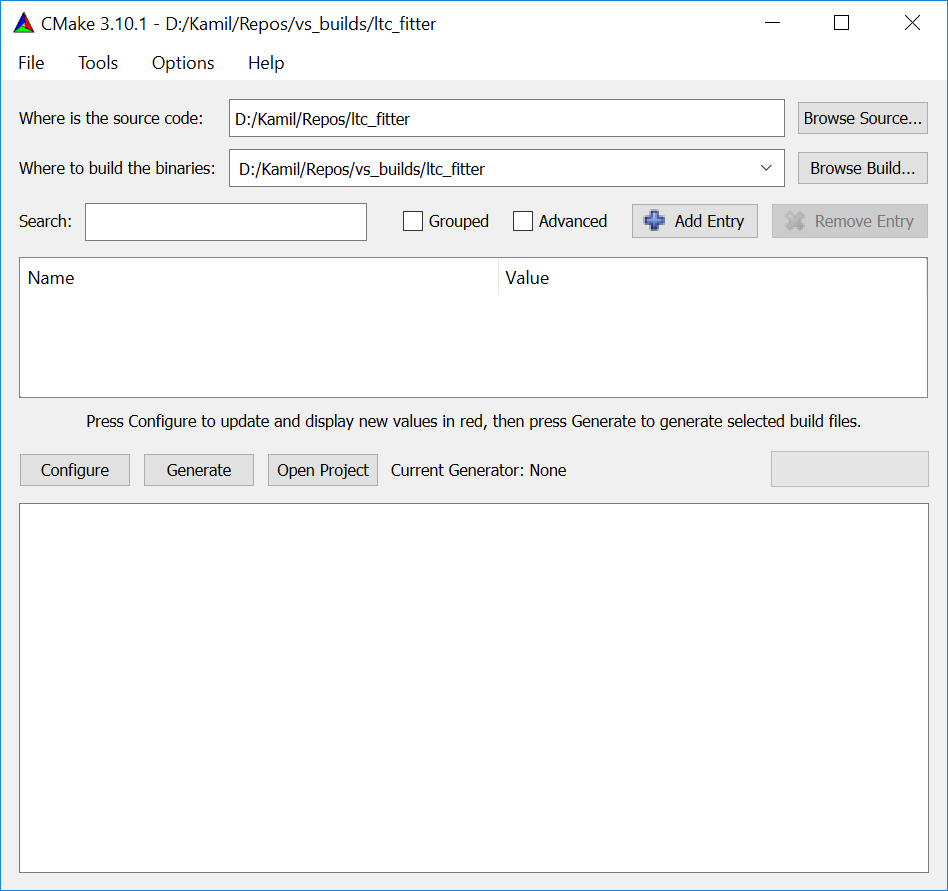
\includegraphics[width=\textwidth]{architecture/cmake/gui-step-1}
        \caption{Wybieramy katalog główny kodu źródłowego w którym znajduje się plik \texttt{CMakeLists.txt} oraz katalog w którym zostaną umieszczone pliki projektu. Klikamy ,,Configure''.}
    \end{subfigure}
    \hspace{0.5cm}
    \begin{subfigure}[t]{0.40\textwidth}
        \centering
        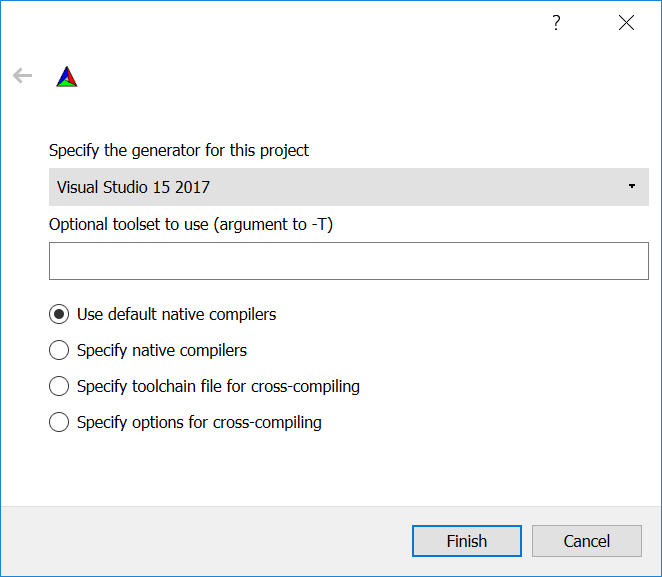
\includegraphics[width=\textwidth]{architecture/cmake/gui-step-2}
        \caption{Wybieramy narzędzie dla którego projekt zostanie wygenerowany, tutaj wybraliśmy ,,Visual Studio 2017''.}
    \end{subfigure}

    \hfill \\ 
    \vspace{0.5cm}

    \begin{subfigure}[t]{0.40\textwidth}
        \centering
        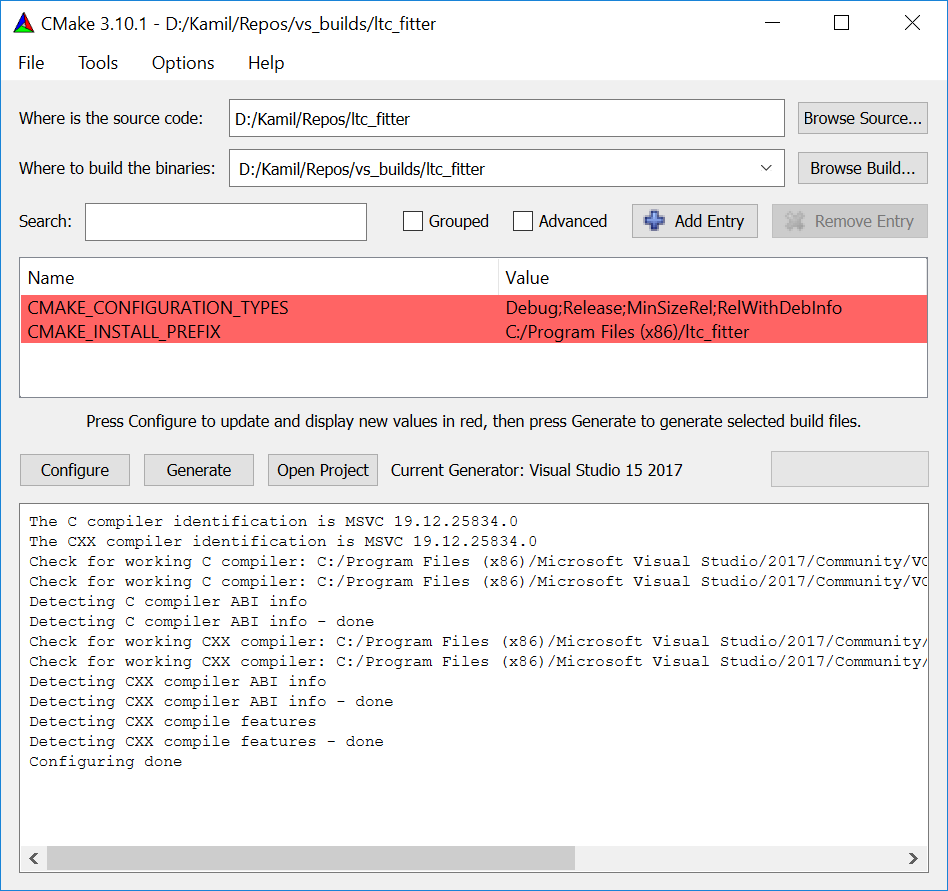
\includegraphics[width=\textwidth]{architecture/cmake/gui-step-3}
        \caption{Po wstępnej konfiguracji pojawiają nam się możliwe opcje do ustawienia, pozostawiamy wszystkie domyślne wartości oraz klikamy ponownie ,,Configure'', następnie ,,Generate''}
    \end{subfigure}
    \hspace{0.5cm}
    \begin{subfigure}[t]{0.40\textwidth}
        \centering
        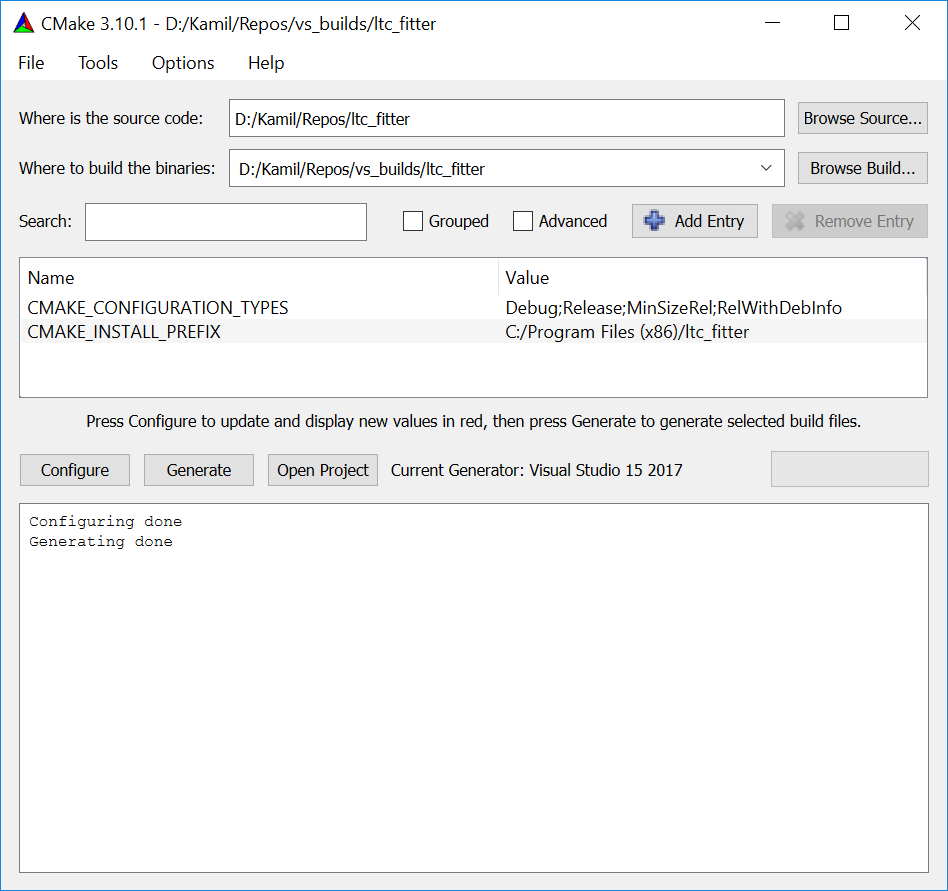
\includegraphics[width=\textwidth]{architecture/cmake/gui-step-4}
        \caption{Projekt został wygenerowany. Po przyciśnięciu ,,Open Project'' powinno otworzyć się IDE w którym możemy skompilować projekt.}
    \end{subfigure}
    
    \caption{Generowanie projektu przy użyciu CMake GUI 3.10.1. Opracowanie własne.}
    \label{fig:CMakeGUIUsage}
\end{figure}


\subsection{Struktura kodu źródłowego}

W główym katalogu repozytorium znajdziemy poszczególne pliki oraz katalogi zawierające wszystko co jest potrzebne do uruchomienia aplikacji.

\begin{description}
    \item[\texttt{CMakeLists.txt}] \hfill\\ 
    plik opisujący sposób generowania projektów dla poszczególnych IDE 
    
    \item[\texttt{README.md}] \hfill\\ 
    krótki opis aplikacji i podstawowy sposób użytkowania 
    
    \item[\texttt{scripts/}] \hfill\\ 
    skrypty pomocnicze do generowania podglądów i wyszukiwania błędów
    
    \item[\texttt{src/}] \hfill\\ 
    katalog ze źródłami aplikacji
    
    \item[\texttt{dependencies/}] \hfill\\ 
    katalog ze źródłami zależności aplikacji, znajdują się tam źródła biblioteki \texttt{glm} \cite{GLMProject} do operacji na wektorach oraz \texttt{stb} \cite{STBProject} do operacji na mapach bitowych
\end{description}

\noindent W katalogu \texttt{src/} znajdziemy kilka katalogów oraz plików z całą funkcjonalnością aplikacji podzielone ze względu na zastosowanie:

\begin{description}
   
    \item[\texttt{brdf/}] \hfill\\
    definicje BRDF, klasy wewnątrz implementują modele wyznaczające wartość $f_r$ dla danego zbioru parametrów: chropowatości $\alpha$, kierunku obserwacji $\omega_o$ oraz kierunku padania światła $\omega_i$
    
    \item[\texttt{exporters/}] \hfill\\
    klasy transformujące dane z postaci używanej wewnątrz aplikacji do formy optymalnej do przekazania do zapisu przez klasy z katalogu \texttt{files/}
    
    \item[\texttt{files/}] \hfill\\ 
    funkcjonalność wejścia-wyjścia, klasy wewnątrz potrafią wczytywać oraz zapisywać pliki podglądu na niskim poziomie
    
    \item[\texttt{fitting/}] \hfill\\
    zbiór klas organizujących dopasowywanie rozkładu lambertowskiego do danego rozkładu opisanego przez BRDF dla danych parametrów
    
    \item[\texttt{ltc/}] \hfill\\
    klasy pozwalające na przeprowadzanie obliczeń na przekształconych liniowo rozkładach kosinusowych, zawiera także funkcjonalność obliczania błędu między rozkładem LTC, a BRDF
     
    \item[\texttt{numerical/}] \hfill\\
    funkcje numeryczne ogólnego zastosowania: metoda pełzającego sympleksu dla dowolnego wymiaru, generowanie losowych próbek, podstawowe estymatory z funkcją błędu dla ograniczeń
    
    \item[\texttt{plotting/}] \hfill\\
    funkcje generujące podgląd dla BRDF i LTC dla danych parametrów, generowanie podglądów pozwala na szybszą analizę dokładności i naprawianie błędów implementacyjnych
    
    \item[\texttt{tests/}] \hfill\\
    katalog z bardzo prostymi testami dymnymi oraz eksporterem podglądów dla wyników otrzymanych przez \cite{ltc_heitz} 
    
    \item[\texttt{utils/}] \hfill\\
    stałe i funkcje, które nie wpasowały się do pozostałych modułów
\end{description}

\subsection{Architektura aplikacji}

Sercem programu jest elastyczna implementacja algorytmu pełzającego sympleksu z możliwością uruchomienia go w wariancie z funkcją kary. Diagram klas zawierający kluczowe elementy do zrozumienia architektury dopasowywania funkcji znajduje się na rys. \ref{fig:FunctionSolveClassDiagram}. 

Znalezienie parametrów opowiadającym minimum dla danej funkcji wymaga implementacji interfejsu \texttt{error\_estimator}, klasa ta wyznacza wartość błędu dla danych parametrów. Błąd ten minimalizowany jest w trakcie poszukiwania rozwiązania optymalnego. W przypadku funkcji kary, istnieje konieczność wyznaczenia wartości ograniczeń, które potem są przeliczane na dodatkowy, karny błąd zastosowany przez estymator \texttt{penalty\_error\_estimator}. 

\begin{figure}[h]
    \centering
    
\includegraphics[scale=\graphvizscale]{architecture/ltcfitter/fitting.pdf}
    \caption{Wybrane elementy klas dotyczących procesu optymalizacji funkcji. Opracowanie własne.}
    \label{fig:FunctionSolveClassDiagram}
\end{figure}

W celu wykonania obliczeń koniecznych do znalezienia macierzy $M$ transformującej rozkład kosinusowy do postaci bliskiej rozkładowi referencyjnemu musimy dodać kilka elementów do powyższej struktury. Dzięki interfejsom, dodanie rozszerzeń jest bardzo proste. Pierwszym krokiem, jest implementacja BRDF referencyjnego, w naszym przypadku GGX (rys. \ref{fig:BRDFClassDiagram}).

\begin{figure}[h]
    \centering
    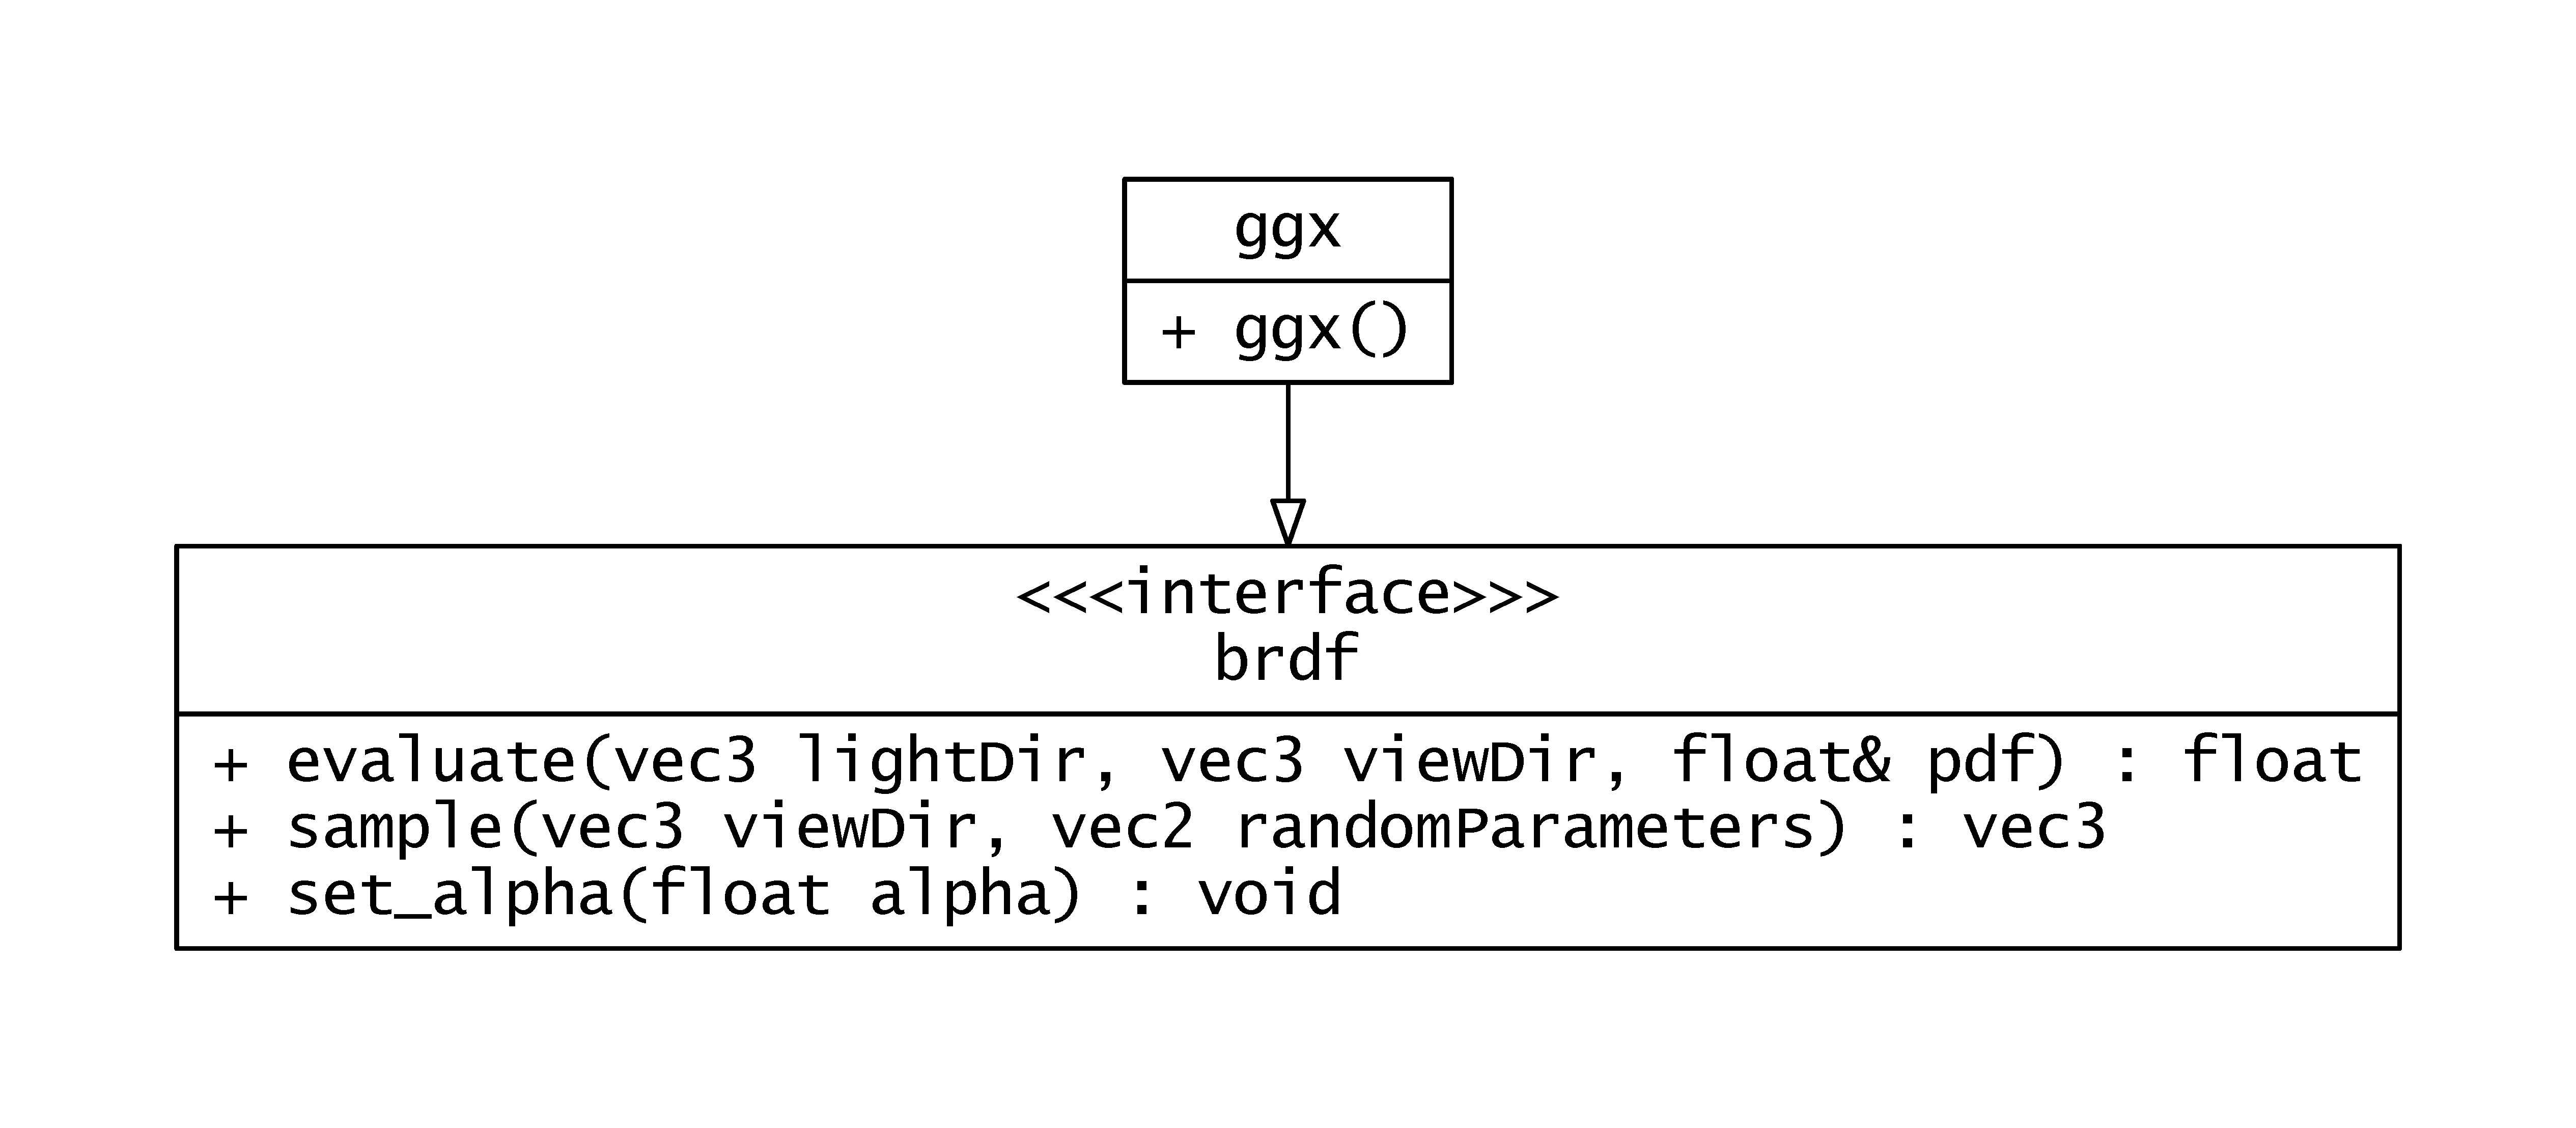
\includegraphics[scale=\graphvizscale]{architecture/ltcfitter/brdf.pdf}
    \caption{Interfejs \texttt{brdf} standaryzujący operacje na modelach BRDF. Opracowanie własne.}
    \label{fig:BRDFClassDiagram}
\end{figure}

Kolejnym krokiem jest implementacja kolejno: 
\begin{enumerate}
    \item reprezentacji liniowo transformowanych kosinusów, którą będziemy traktować jak BRDF,
    \item estymator błędu między obecnym przybliżeniem, a BRDF referencyjnym,
    \item kalkulator ograniczeń, które zostaną wykorzystane do nałożenia kary w przypadku zbliżenia się do granic.
\end{enumerate}

Implementacja już istniejących interfejsów (rys. \ref{fig:LTCClassDiagram}) pozwoli nam na wykorzystanie w pełni mechanizmu wyszukiwania minimum funkcji do znalezienia optymalnej transformacji.

\begin{figure}[h]
    \centering
    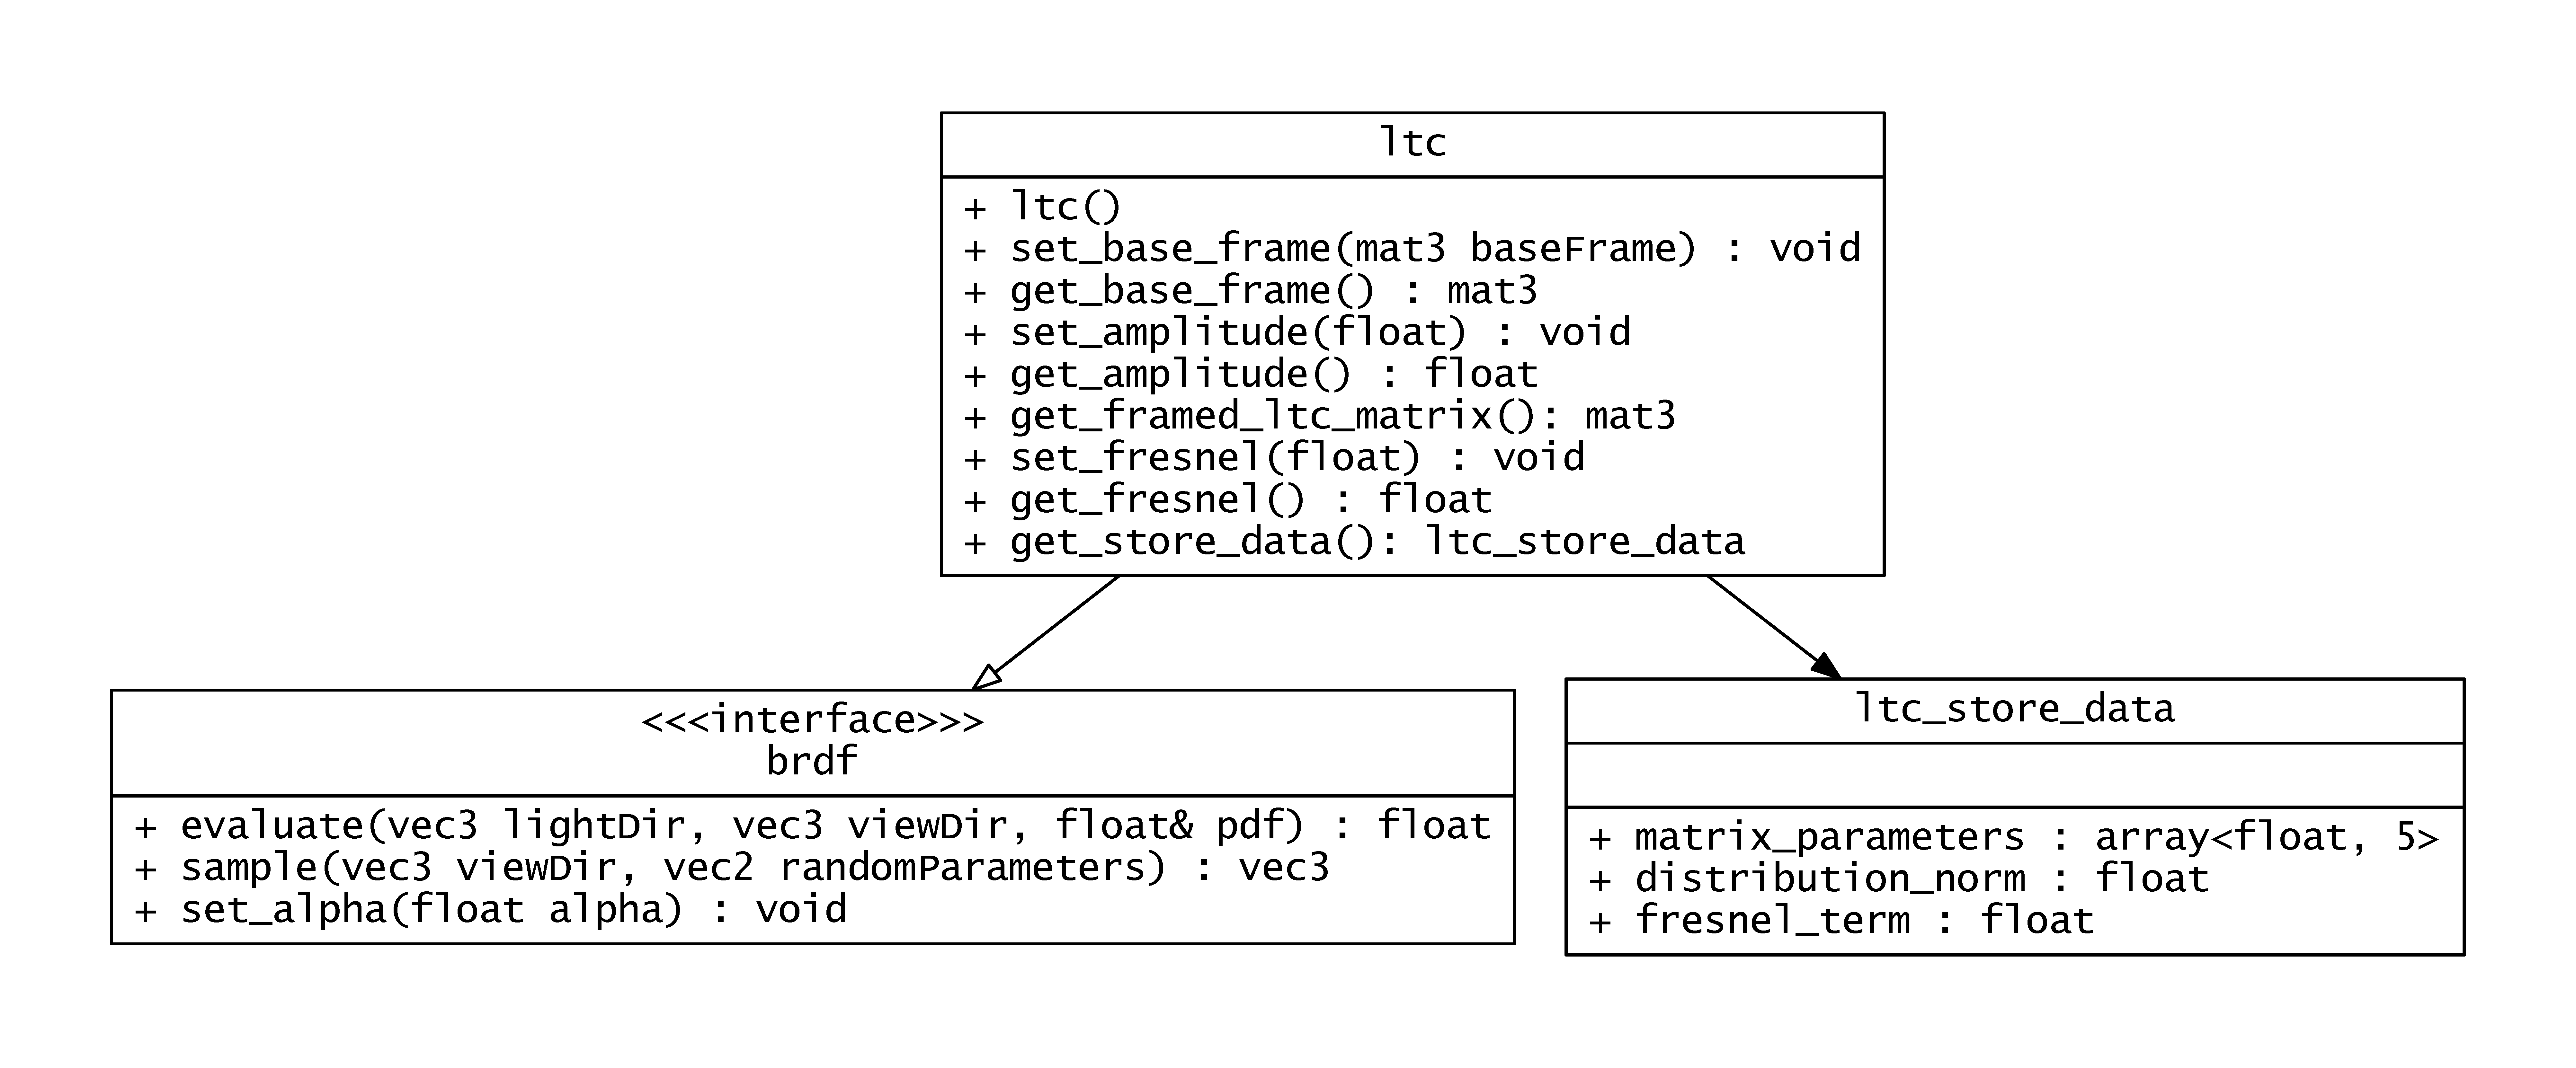
\includegraphics[scale=\graphvizscale]{architecture/ltcfitter/ltc1.pdf}
    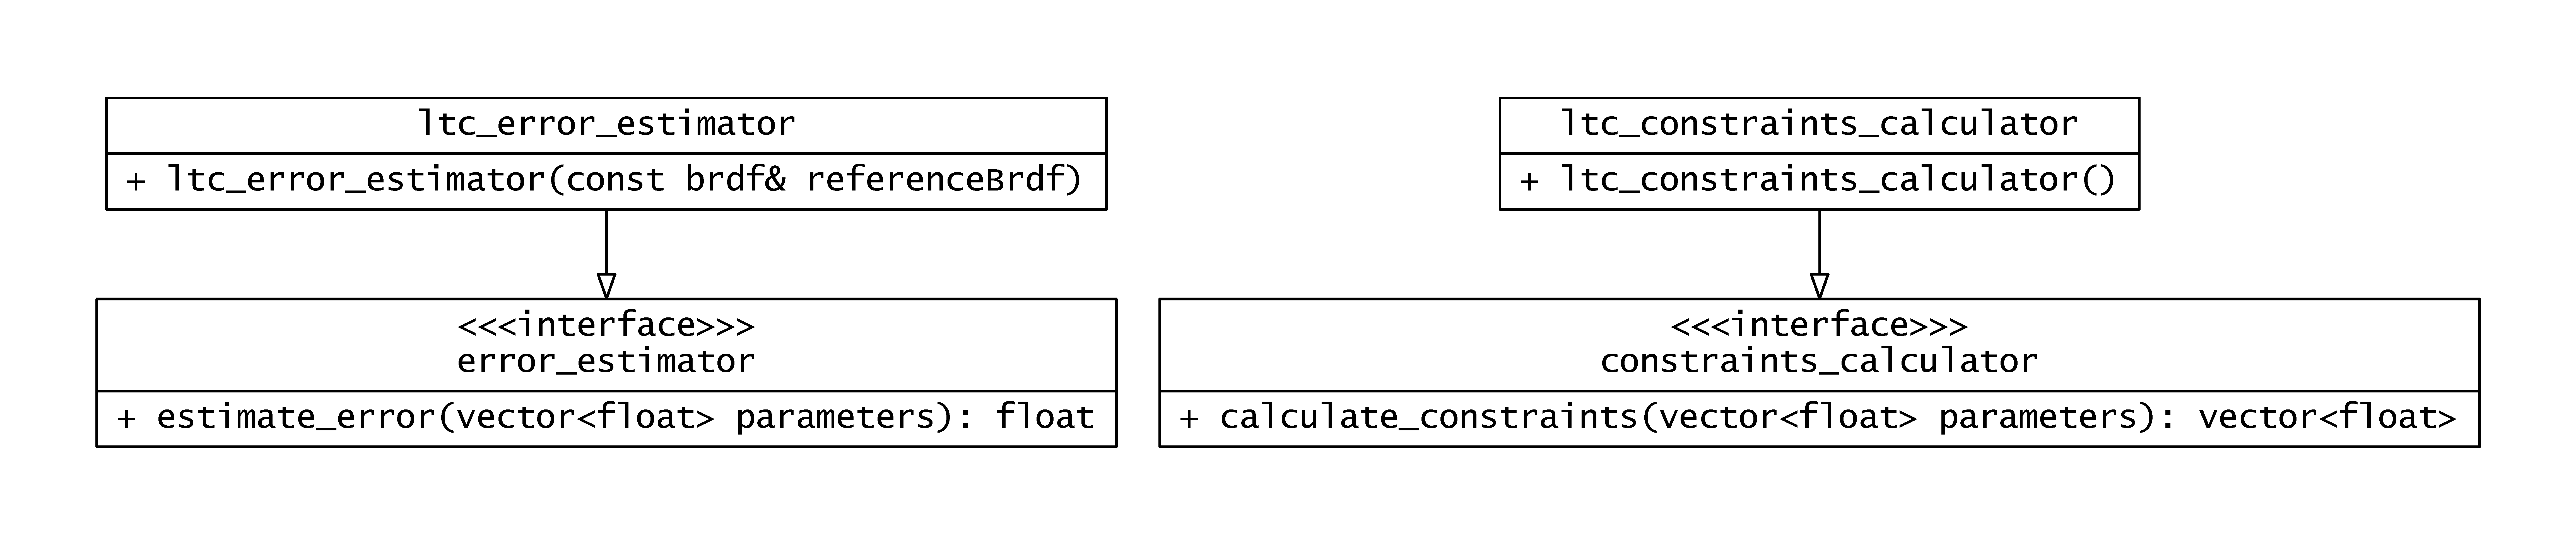
\includegraphics[scale=\graphvizscale]{architecture/ltcfitter/ltc2.pdf}
    \caption{Klasy implementujące wsparcie dla optymalizacji macierzy $M$ dla metody LTC. Opracowanie własne.}
    \label{fig:LTCClassDiagram}
\end{figure}

Procedurę wyznaczania parametrów wejściowych dla BRDF referencyjnego oraz ich zapisu do pliku możemy znaleźć w funkcji \texttt{build\_lookup}. Funkcja ta, dzieli dziedzinę na zadaną liczbę próbek, znajduje przybliżone rozwiązanie początkowe i uruchamia funkcję \texttt{ltc\_fit}, która z kolei buduje drzewo zależności wymagane przez algorytm pływającego sympleksu i znajduje optymalne rozwiązanie dla danych parametrów wejściowych.

\subsection{Format plików wyjściowych}


Plik wyjściowy został zoptymalizowany w taki sposób, by jego wczytanie do pamięci karty graficznej nie wymagało żadnych modyfikacji danych. Plik ten możemy podzielić na trzy części: nagłówek, teksturę pierwszą i drugą.

Nagłówek składa się z kilku pól opisujących zawarte dane oraz wersję pliku. Jego struktura przedstawiona jest w tabeli \ref{tab:alf_header}.

\begin{table}[h]
    \centering
    \begin{tabular}{|l|l|l|}
        \hline
        Typ & Rozmiar (bit) & Opis \\ \hline 
        \texttt{char[4]} & $4*1=4$ & Ustalona wartość kontrolna równa ,,ALFS'' \\ \hline
        \texttt{short} & $16$ & Numer główny wersji (ang. \textit{major}) \\ \hline
        \texttt{short} & $16$ & Numer dodatkowy wersji  (ang. \textit{minor}) \\ \hline
        \texttt{uint} & $32$ & Liczba próbek ze względu na kąt (ozn. $n$) \\ \hline
        \texttt{uint} & $32$ & Liczba próbek ze względu na chropowatość (ozn. $m$) \\ \hline
    \end{tabular}
    \caption{Struktura nagłówku pliku wynikowego.}
    \label{tab:alf_header}
\end{table}

Zaraz po nagłówku rozpoczynają się dane pierwszej tekstury. Oznaczmy liczbę próbek ze względu na kąt $n$ i liczbę próbek ze względu na chropowatość $m$. Dane pierwszej tekstury zawierają $nm$ rekordów zawierających wynik dla danego kąta i chropowatości o równym rozmiarze. Pozycję $p$ dla danej próbki dla $i$-tego podziału kąta i $j$-tej wartości chropowatości ($0 \leq i < n$, $0 \leq j < m$) opisuje równanie (\ref{eq:alf_position}). Każdy z rekordów na danej pozycji ma strukturę opisaną w tabeli \ref{tab:alf_ts1_value}.

\begin{equation}
  p(i,j) = m * i + j
  \label{eq:alf_position}
\end{equation}

\begin{table}[h]
    \centering
    \begin{tabular}{|l|l|l|}
        \hline
        Typ & Rozmiar (bit) & Opis \\ \hline 
        \texttt{float} & $32$ & Współczynnik $M_0^0$ znalezionej macierzy wynikowej \\ \hline
        \texttt{float} & $32$ & Współczynnik $M_0^2$ znalezionej macierzy wynikowej \\ \hline
        \texttt{float} & $32$ & Współczynnik $M_1^1$ znalezionej macierzy wynikowej \\ \hline
        \texttt{float} & $32$ & Współczynnik $M_2^0$ znalezionej macierzy wynikowej \\ \hline
    \end{tabular}
    \caption{Struktura próbki w teksturze pierwszej.}
    \label{tab:alf_ts1_value}
\end{table}

Dane drugiej tekstury znajdują się od razu po danych pierwszej tekstury. Rekordy ułożone są w identyczny sposób jak w teksturze pierwszej, ale każdy z nich ma inną strukturę, opisaną w tabeli \ref{tab:alf_ts2_value}.

\begin{table}[h]
    \centering
    \begin{tabular}{|l|l|l|}
        \hline
        Typ & Rozmiar (bit) & Opis \\ \hline 
        \texttt{float} & $32$ & Współczynnik $M_2^2$ znalezionej macierzy wynikowej \\ \hline
        \texttt{float} & $32$ & Norma rozkładu wejściowego $n_D$ \\ \hline
        \texttt{float} & $32$ & Współczynnik Fresnela otrzymany podczas wyznaczania przybliżenia $f_D$ \\ \hline
    \end{tabular}
    \caption{Struktura próbki w teksturze pierwszej.}
    \label{tab:alf_ts2_value}
\end{table}

%\begin{table}[]
%    \begin{tabular}{|l|l|l|l|l|l|}
%        \hline
%        \multicolumn{2}{|l|}{\multirow{5}{*}{Header}}          & char{[}4{]} & 4*1=4 & File magic number           & Equal to ALFS \\ \cline{3-6} 
%        \multicolumn{2}{|l|}{}                                 & short       & 16    & Major version               & Equal to 1    \\ \cline{3-6} 
%        \multicolumn{2}{|l|}{}                                 & short       & 16    & Minor version               & Equal to 0    \\ \cline{3-6} 
%        \multicolumn{2}{|l|}{}                                 & uint        & 32    & Number of angle samples     &               \\ \cline{3-6} 
%        \multicolumn{2}{|l|}{}                                 & uint        & 32    & Number of roughness samples &               \\ \hline
%        \multirow{6}{*}{Texture Slot \#1} & \multirow{4}{*}{1} & float       & 32    & Matrix coefficient: M00     &               \\ \cline{3-6} 
%        &                    & float       & 32    & Matrix coefficient: M02     &               \\ \cline{3-6} 
%        &                    & float       & 32    & Matrix coefficient: M11     &               \\ \cline{3-6} 
%        &                    & float       & 32    & Matrix coefficient: M20     &               \\ \cline{2-6} 
%        & \multicolumn{5}{l|}{...}                                                               \\ \cline{2-6} 
%        & Number samples     & \multicolumn{4}{l|}{Same format as above.}                        \\ \hline
%        \multirow{4}{*}{Texture Slot \#2} & \multirow{3}{*}{1} & float       & 32    & Matrix coefficient: M22     &               \\ \cline{3-6} 
%        &                    & float       & 32    & Original BRDF magniture     &               \\ \cline{3-6} 
%        &                    & float       & 32    & Fresnel coefficient         &               \\ \cline{2-6} 
%        & \multicolumn{5}{l|}{...}                                                               \\ \hline
%    \end{tabular}
%\end{table}

\section{Program \texttt{arealights}}

Program \texttt{arealights} jest aplikacją graficzną realizującą algorytmy symulujące światła powierzchniowe zamieszczone w tej pracy.

Kod programu można znaleźć na dołączonej płycie CD lub w repozytorium online pod adresem: \url{https://github.com/sienkiewiczkm/arealights}.

\subsection{Opis użytkowania}

Aplikacja przykładowa posiada bardzo prosty interfejs składający się z okna konfiguracyjnego oraz podglądu (rys. \ref{fig:app_arealights_view}). Zmiana ustawień powoduje natychmiastowe zaaplikowanie wartości i odświeżenie podglądu. Akcje i przypisane do nich klawisze przedstawione są w tabeli \ref{tab:arealights_keybindings}.

\begin{figure}[h]
    \centering
    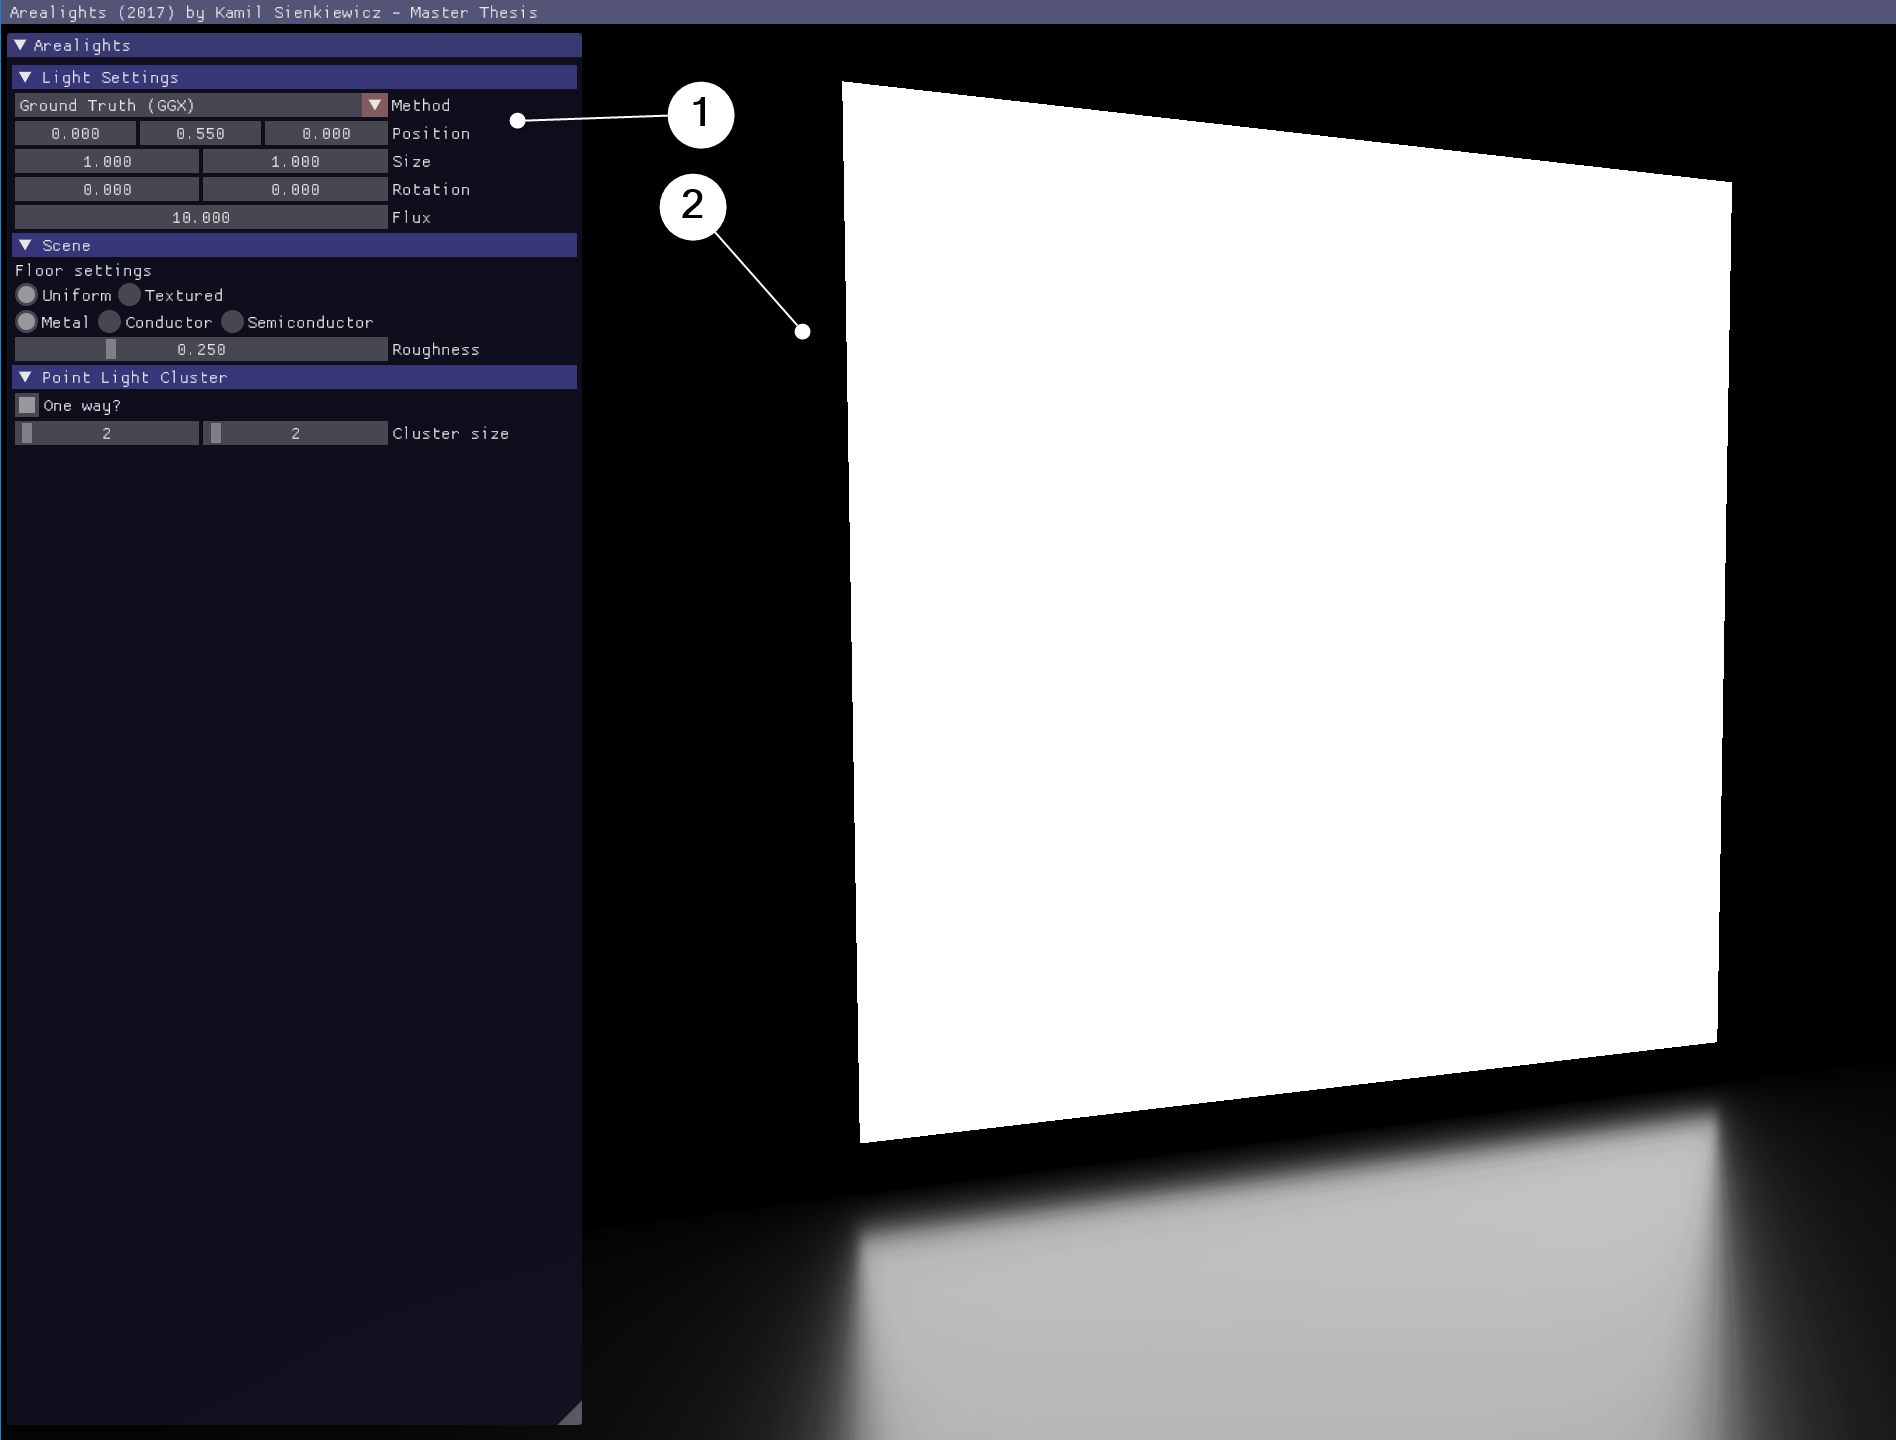
\includegraphics[width=0.7\linewidth]{architecture/arealights_view}
    \caption{Widok główny aplikacji przykładowej. 1) Widok ustawień 2) Podgląd. Opracowanie własne.}
    \label{fig:app_arealights_view}
\end{figure}

\begin{table}[h]
    \centering
    \begin{tabular}{|l|l|}
        \hline \textbf{Przycisk} & \textbf{Akcja} \\ \hline
        W & ruch kamery do przodu \\ \hline
        S & ruch kamery do tyłu \\ \hline
        A & ruch kamery w lewo \\ \hline
        D & ruch kamery w prawo \\ \hline
        lewy przycisk myszki & obrót kamery \\ \hline
        P & zapis podglądu do pliku \texttt{.png} \\ \hline
        L & zablokowanie lub odblokowanie kamery \\ \hline
    \end{tabular}
    
    \caption{Lista akcji przypisanych do przycisków w aplikacji \texttt{arealights}.}
    \label{tab:arealights_keybindings}
\end{table}

Widok ustawień podzielony jest na sekcje: ustawienia światła (ang. \textit{Light settings}), ustawienia sceny (ang. \textit{Scene settings}) oraz ustawienia zależne od wybranej metody oświetlenia.

Ustawienia światła (rys. \ref{fig:app_arealights_light_settings}) umożliwiają wybór jednej z opisanych w tej pracy metod oraz ustawienia światła w scenie oraz zdefiniowanie energii całkowitej źródła.

\begin{figure}[h]
    \centering
    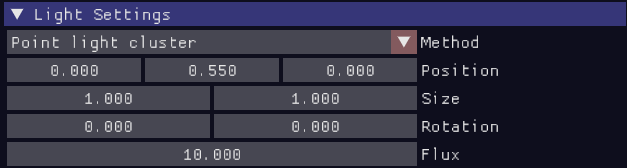
\includegraphics[width=0.7\linewidth]{architecture/arealights/light_settings}
    \caption{Ustawienia światła, kolejno są to: aktualnie używana metoda, pozycja światła prostokątnego, rozmiar źródła, obrót, energia światła.}
    \label{fig:app_arealights_light_settings}
\end{figure}

\subsection{Kompilacja}

Kompilacja tego projektu przebiega analogiczne do poprzedniego programu. Szczegóły dotyczące budowania aplikacji można znaleźć w rozdziale \ref{section:ltcFitterCompilation}.

\subsection{Struktura kodu źródłowego}

W głównym katalogu repozytorium znajdują się poszczególne pliki i katalogi:

\begin{description}
    \item[\texttt{assets/}] \hfill \\ 
    katalogu zawierający tekstury, tablice podglądu wygenerowane przez \texttt{ltc\_fitter} oraz kod programów cieniujących
    
    \item[\texttt{dependencies/}] \hfill \\ 
    katalog ze źródłami zależności
    
    \item[\texttt{source/}] \hfill \\ źródła aplikacji
    
    \item[\texttt{CMakeLists.txt}] \hfill\\ 
    plik opisujący sposób generowania projektów dla poszczególnych IDE 

    \item[\texttt{README.md}] \hfill\\ 
    krótki opis aplikacji i podstawowy sposób użytkowania 
    
\end{description}

\subsection{Architektura aplikacji}


\end{document}